\documentclass[sigconf]{acmart}

\def\BibTeX{{\rm B\kern-.05em{\sc i\kern-.025em b}\kern-.08emT\kern-.1667em\lower.7ex\hbox{E}\kern-.125emX}}
\usepackage{subfigure}
\usepackage{algorithm}
%\usepackage{algorithmic}
\usepackage{algpseudocode}
\usepackage{amsmath}
\usepackage{graphics}
\usepackage{epsfig}
\usepackage{multirow}
\usepackage{graphicx}
\usepackage{subfigure}

\renewcommand{\algorithmicrequire}{\textbf{Input:}} % Use Input in the format of Algorithm
\renewcommand{\algorithmicensure}{\textbf{Output:}} % Use Output in the format of Algorithm

\begin{document}

\title{Approximate Code: A Cost-Effective Erasure Code for Video Applications in Cloud Storage Systems}

\author{Huayi Jin}


%-------------------------ATTANTION-------------------------%
%                                                           %
% orange words show the content that requires to be add     %
% blue words need to be perfected or changed                %
% gray words are the placeholder which is easy to fill      %
%                                                           %
%-----------------------------------------------------------%

\begin{abstract}
Multimedia data generated by autonomous driving, media industry and security monitoring is often stored in cloud storage systems and occupies a large amount of space. Meanwhile, to ensure the data reliability, distributed file systems often use erasure codes to backup data. However, the commonly used triple disk failure tolerant arrays (3DFTS) erasure code scheme is expensive, not only because simultaneous damage of multiple disks is relatively rare, but also due to its ignorance of redundant information inside the data, resulting in multiple complete parity disks being excessive. On the other hand, the recently proposed approximate storage scheme can effectively reduce storage costs, but at the cost of sacrificing the reliability of some data.

In this article, we propose Approximate Code for multimedia applications, which is an erasure code using an approximation strategy. Approximate Code aims to ensure different reliability of important and unimportant data by means of erasure coding, thereby reducing storage overhead. It provides complete recovery when fewer disks fail, and ensures approximate recovery (recover most data) in the event of multiple disk failures. To demonstrate the effectiveness of Approximate Code, we conduct several experiments in Hadoop and Alibaba Cloud systems. 
The results show that compared with the typical high-reliability erasure code schemes, Approximate Code significantly reduces reduce the storage overhead and provide high reliability of important data.

\end{abstract}

%
% The code below is generated by the tool at http://dl.acm.org/ccs.cfm.
% Please copy and paste the code instead of the example below.
%
\keywords{Erasure Codes, Approximate Storage, Multimedia, Cloud Storage}

\maketitle

\section{Introduction}
Multimedia data consumes massive storage space in cloud storage systems, and this trend is exacerbated as applications demand higher resolution and frame rates. On YouTube, nearly 140,000 hours of video are played every minute and 400 hours of video are uploaded. Rapidly growing data imposes very high requirements of reliability and availability on large-scale storage systems as well as low cost.

Although multiple replicas can be used to ensure data availability and reliability, this method is too expensive and is only used to save hot data in practice. In contrast, the amount of cold data is far more than hot data, and erasure code (EC) schemes are ideal for storing such data. It provides lower storage overhead and write bandwidth than replication with the same fault tolerance. Currently, many cloud storage systems use erasure code to tolerate disk failures and ensure data availability, such as Windows [], Amazon AWS [] or Alibaba Cloud []. Typical erasure codes configuration use three-disk fault tolerant array (3DFTS). However, its overhead is still too high because the simultaneous damage of triple disks is relatively rare. 

The recently proposed approximate storage strategy can significantly reduce the consumption of storage resources and energy. Common methods are to ensure the reliability of important data while storing the unimportant data on relatively unreliable media or reducing their error correction coding. Multimedia data is a typical application scenario for approximate storage because they can tolerate data corruption compared to other data. For example, video data records at least 20 frames per second, which makes it difficult for a typical user to perceive the loss of several frames. Also, some pixel errors in the image data do not affect the information of the entire picture. However, the direct application of approximate storage in a cloud storage system will result in the unimportant data being unacceptable volatile.

//////////////////////

Therefore, we propose Approximate Codes for multimedia data that reduce storage overhead by reducing the parity of data that is not sensitive to errors. In the scenario shown in Figure \ref{fig-Ap-322}, the Approximate Codes are designed for systems composed of $n$ disks where $m$ disks are dedicated to coding.
Other $s \times t$ sectors are encoded for important data thus raise its reliability. Approximate Codes ensure that the important data can tolerate $m+s$ device failures while all data can tolerate $m$ device failures.
When more than $s$ disks fails, Approximate Code recovers the important data and then transfer the surviving data to the upper layer for recovery. 

//////////////////////

With proper data distribution and algorithm design, the quality loss of video or image can be controlled within an acceptable range of applications, which leads to another important task in approximating storage, distinguishing data importance.
This work is traditionally done by experienced programmers. Fortunately, multimedia data is commonly compressed and stored in encoded formats, which results in a certain portion of such data being more important than others. For example, in the progressive transform codec (PTC) compressed image, control and run-length bits are much more important than refinement bits. Therefore, this work can be done automatically by a system tailored to specific encodings.

Our work contributions include:
\begin{enumerate}
\item We propose Approximation Code that reduces storage overhead and improves the reliability and availability of important data with the approximate strategy.
\item We prove the mathematical correctness of the Approximation Code.
\item We perform a series of experiments and show that Approximate Code performs better than the traditional method in the full recovery mode, and the data loss in the approximate mode is acceptable.
\end{enumerate}

The rest of the paper is organized as follows. In Section \ref{RelatedWork}, we introduce related work and our motivation. 
In Section \ref{ApCode}, the design of Approximate Code and its encoding and decoding process will be illustrated in detail. 
Section \ref{Implementation} introduce the implementation of our design.
The evaluation is presented in Section \ref{evaluation} and the conclusion of our work is in Section \ref{Conclusion}. 


\section{Related Work and Our Motivation}\label{RelatedWork}
This section presents background on erasure codes, related video storage methods, approximate storage, and our motivation.

\iffalse
\begin{table}[]
\begin{tabular}{|c|l|}
\hline
Symbols & Description                          \\ \hline\hline
$n$     & the number of chunks in a stripe     \\ \hline
$m$     & the number of parity chunks          \\ \hline
$r$     & the number of sectors in a chunk     \\ \hline
$s$     & the number of columns of $D_I$       \\ \hline
$t$     & the number of rows of $D_I$          \\ \hline
$D_I$   & the zone of important data sectors   \\ \hline
$D_M$   & the zone of unimportant data sectors       \\ \hline
$Q$     & the zone of important parity sectors \\ \hline
$P$     & the zone of unimportant parity sectors     \\ \hline
\end{tabular}
\end{table}
\fi

\subsection{Existing Erasure Codes}

\begin{figure}[ht]
\centering
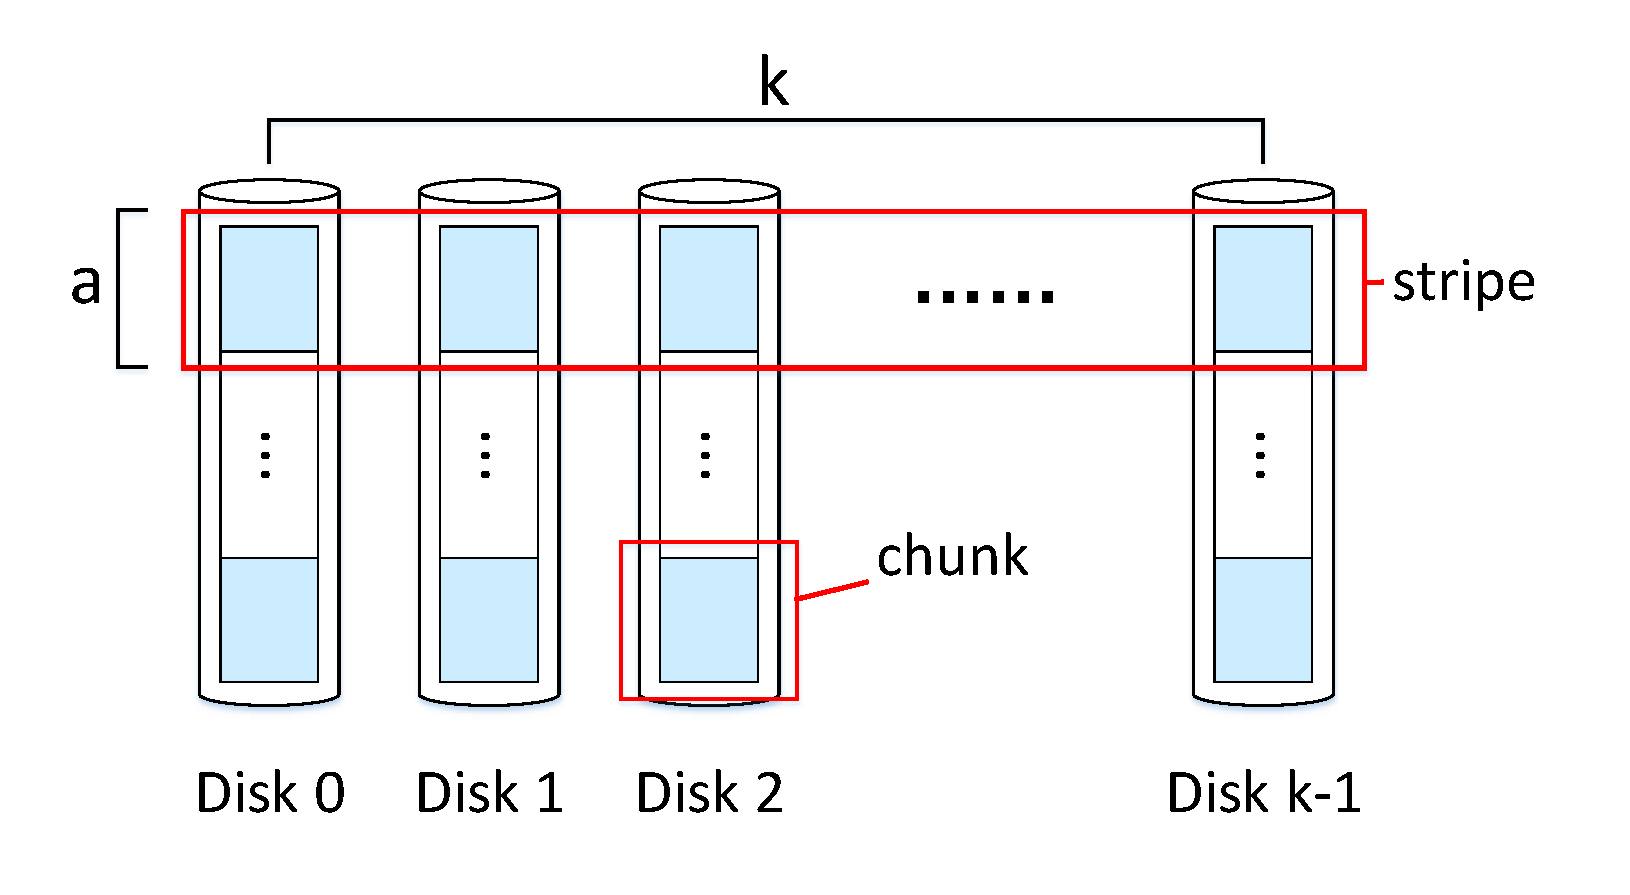
\includegraphics[width=0.3\textwidth]{photo/chunk.pdf}
\caption{A sample of chunks and stripes}
\label{fig-chunk}
\end{figure}


Reed Solomon Code (RS code) is a kind of Maximum Distance Separable (MDS) Codes, which have the optimal storage efficiency. The encoding and decoding operations of RS code are based on Galois Field, which leads to a higher computational complexity comparing to XOR-based codes.

However, due to its high scalability, RS code has been widely applied in traditional cloud storage systems. In a RS code which is delegated by RS($k$, $r$), $n = k + r$ denotes the total number
of nodes participating in the erasure coding schema, $k$ stands for the number of data nodes, and $r$ is the number of parity nodes. Generally data is organized and encoded/decoded with the minimum coding unit block. RS($k$, $r$) can tolerate at most $r$ failures at the same time, and single node failure can be recovered from any $k$ survivors. The encoding case of RS code and the failure tolerance processus are shown in Figure 1.


\begin{figure}[ht]
\centering
\begin{minipage}[b]{0.3\textwidth}
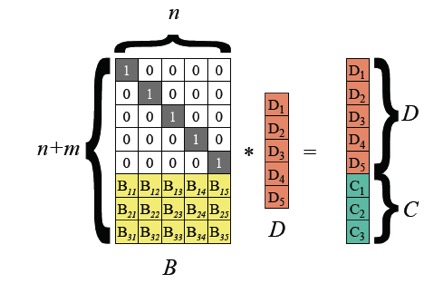
\includegraphics[width=0.52\textwidth]{photo/RS1.jpg}
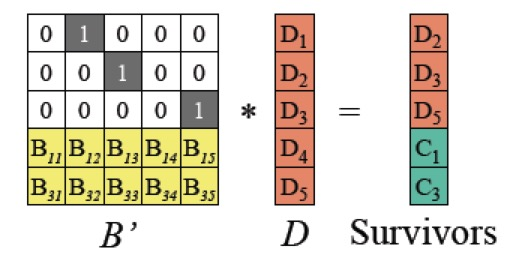
\includegraphics[width=0.4\textwidth]{photo/RS2.jpg}
\end{minipage}
\caption{Encoding process of RS($5$, $3$)}
\end{figure}

\begin{figure}[H]
\centering
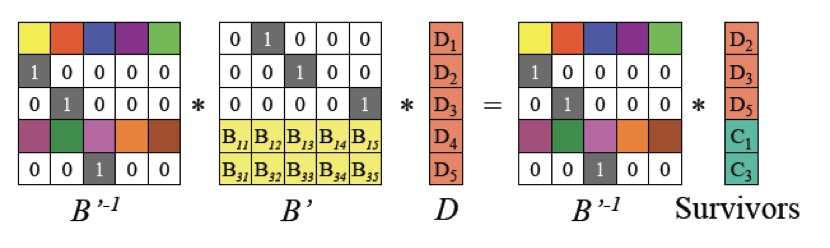
\includegraphics[width=0.3\textwidth]{photo/RS3.jpg}
\caption{Recovery processing of RS($5$, $3$) in the case of 3 random failure}
\end{figure}

\textcolor{red}{In our case, RS code could be applied. As the important data are uniformly-distributed in every node, the data in every node could be considered independent to each other. The principal of video storage divides the data into a small part of important frame and other subordinate frames. If a storage failure occurs in a node that stores largely the important frame, the data recovery may not be complete because the loss of the important frame could lead to a video quality degradation. In this way, this kind of uniformly-distribution would not allow the failure causing the data loss bigger than expected.}

\textcolor{red}{The data distribution assures the independency of nodes, the recovery of data could follow nearly the theoretical case. The recovery processus need the reversible matrix of original matrix. The calculation is shown in Figure 2.}

Another type of erasure code worth mentioning is XOR based codes, which uses purely XOR operations. There are two different approaches to implement XOR codes. One is to use generator matrix\cite{plank2004practical} for encoding/decoding operations, and the other is done by using specific algorithm for each code\cite{huang2008star}. In nowadays cloud storage systems, erasure codes for correcting two or three disk failures are widely used to ensure the reliability, and XOR-based codes show great advantages on encoding/decoding speed when the storage system is recovering from failures. XOR-based codes can be further categorized as XOR-based codes used in RAID-6 and ones to backup triple disk failure.

When it comes to RAID-6, Maximum Distance Separable (MDS) \cite{jin2009p} \cite{cassuto2009cyclic} \cite{blaum1999lowest} \cite{corbett2004row} \cite{blaum1995evenodd} \cite{bloemer1995xor} codes are frequently discussed. There are two types of MDS codes with different properties. One of them is called horizontal MDS codes, but it suffers from high write complexity and unbalanced I/O distribution. Accordingly, the other is called vertical MDS codes which has a common disadvantage of having resource-consuming partial strip write to continuous data.

A novel and efficient XOR-based RAID-6 code, named hybrid code(h-code) \cite{inproceedings}, is introduced a few years ago. This type of codes exploits the benefits of both horizontal and vertical MDS codes, therefore achieving optimization of partial stripe writes for RAID-6 in addition. H code can be applied to any array of (p+1) disks, where p is a prime number. The parities in H-Code are typical row parity and anti-diagonal parity. H-code does not have a specialized anti-diagonal parity strip, while it distributes the anti-diagonal parity elements among all the disks. Its horizontal parity ensures a partial stripe write to continuous data elements in a row share the same row parity chain, which achieves optimal partial stripe write performance. H code can be applied to any array of (p+1) disks, where p is a prime number. The analysis shows that H-Code achieves excellent performance in storage efficiency, encoding/decoding computational complexity and single write complexity. 


\subsection{Video Storage}\label{video storage}
For normal HD (resolution 1280$\times$720, 8-bit, 30 fps) video, the amount of raw video data in 1 minute is 4.63 GB, so video data is usually encoded and compressed before storage. Lossy compression is a common method that provides a much lower compression ratio than lossless compression while ensuring tolerable loss of video quality, and that is why we focus on such algorithms.


H.264 is one of the advanced algorithms for this type of work. This coding technique is widely used on platforms such as YouTube because it has higher compression ratio and lower complexity than its predecessor. For the HD video mentioned earlier, H.264 can reduce its size by about 10 times, only 443.27MB.

H.264 classifies all frames into three different categories:
\begin{enumerate}
    \item I frame: A frame that does not depend on other frame data, which means it can be decoded independently of other frames.
    \item P frame: A frame holds the changes compared to the previous frame, thus saving much space by leaving out redundant information.
    \item B frame: A frame saves more space by utilizing the data of both the preceding and following frame.
\end{enumerate}
In order to prevent the circumstance where a P or B frame references another distant frame, the concept of GOP is introduced. A GOP consists of multiple consecutive I,P and B frames which are independent of the frames in other GOPs. In other words, a P or B frame can only reference the ones inside the GOP which it belongs to, as shown in Figure \ref{H264-IPB}.
\begin{figure}[ht]
\centering
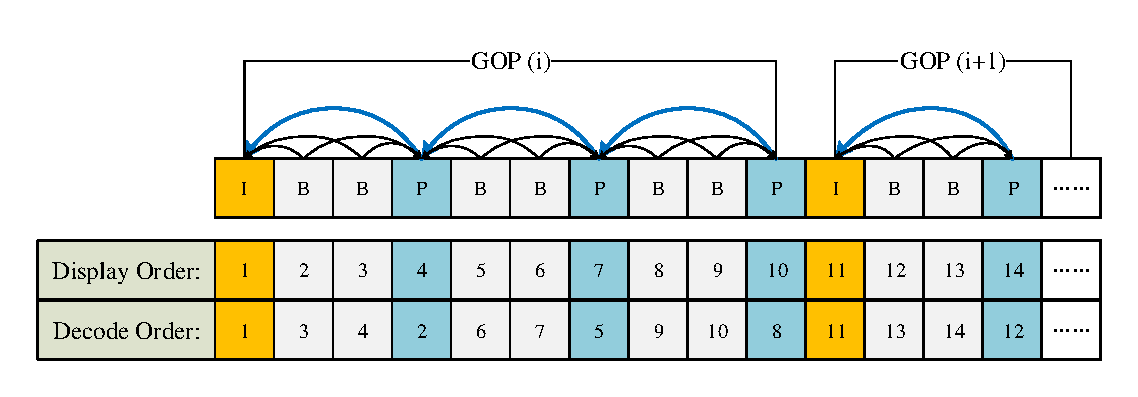
\includegraphics[width=0.45\textwidth]{photo/H264_IPB.pdf}
\caption{A sample of GOPs in H.264}
\label{H264-IPB}
\end{figure}


\subsubsection{Video Frame Recovery}

In the circumstance of video approximate storage, it's common to lose some frames and leave the video incomplete. However, the lost frames may still be recoverable with the benefit of nowadays powerful deep learning techniques. One of them is named video frame interpolation.

Video frame interpolation is one of the basic video processing techniques, an attempt to synthetically produce one or more intermediate video frames from existing ones, the simple case being the interpolation of one frame given two consecutive video frames. This is a technique that can model natural motion within a video, and generate frames according to this modelling. Artificially increasing the frame-rate of videos enables the possibility of frame recovery.


In deep learning methods, optical changes between the frames are trained in a supervised setup mapping two frames to their ground truth optical flow. Among all these, a multi-scale network\cite{van2017frame} based on recent advances in spatial transformers and composite perceptual losses as well as a context-aware Synthesis approach\cite{niklaus2018context} have so far produced the new state-of-the-art results in terms of PSNR and middlebury benchmark respectively.


The methods are relied on the completeness of some video frame, which enhances the importance of the only intact type of frame data in commonly used H.264 standard: the I frame.


\subsection{Approximate Storage}
Storage techniques nowadays generally regard all information of the same importance, which causes significant costs in energy, disk drives and computing resources. But not all data need high-reliability storage for its backup. That is when the concept of approximate storage is introduced. Approximate Storage is another way outside of traditional methods of trading off the limited resource budget with the costly reliability requirements, which recently receives more attentions since data centers are faced with storage pressure from the ever-increasing data.

Use cases for approximate storage range from transient memory to embedded settings and mass storage cloud servers. Mapping approximate data onto blocks that have exhausted their hardware error correction resources, for example, to extend memory endurance. On embedded settings, it enables the reduction of the cost of accesses and preserve battery life to loosen the capacity constraints. \cite{sampson2014approximate} Here, in data-center-scale video database, approximate storage can provide multiple levels of fault tolerance for data of different importance, avoiding redundant backup for the less-important data, thus saving a significant amount of space.


Approximate storage loosens the requirement of storage reliability by allowing quality loss of some specific data. Therefore, programmers can specify the importance of the data segments and assign them to different storage blocks. The critical data is still safe because they are stored and sufficiently backed up by expensive and highly reliable storage devices. Meanwhile, non-critical data is exposed to error, thus increasing storage density and saving cost.


However, it is too naive to store data in approximate storage units indiscriminately. Related research \cite{guo2016high} shows that this can lead to unacceptable data pollution. To ensure data quality in this case, higher error correction costs are required resulting in an increase in overall storage costs.


In the storage of video data, as described in \ref{video storage}, the I frame is the key to decoding the entire GOP. An error in the I frame will cause a decoding error in the P frames and the B frames, and the data loss of the I frame will cause the entire GOP to fail. In contrast, the error or loss of a P frame has less impact, while the B frame is most tolerant of errors because no other frames depend on it.

Considering the vital role the I frame plays in the video coding, we therefore define I frame data as the critical data of a video file. Although some part of P frames may play a relatively important role in the decoding process of a video, it’s importance can not exceed that of the I frames.

\begin{table}[ht]
\centering 
\caption{Comparison of fault tolerance and storage overhead between approximate storage, EC and Approximate Code}\label{tab-AS-EC-AP}
\begin{tabular}{|c|c|c|c|c|}
\hline
\multicolumn{2}{|c|}{Schemes}  & \begin{tabular}[c]{@{}c@{}}Storage\\ Overhead\end{tabular} & Realibilities & Performance \\ \hline\hline
\multirow{2}{*}{EC} & RS & high & high & medium \\ \cline{2-5} 
\multicolumn{1}{|c|}{} & RAID 6 & medium & medium & high \\ \hline
\multicolumn{2}{|c|}{Ap-Storage}& low & very low & high \\ \hline
\multirow{2}{*}{Ap-Code}& Imp & \multirow{2}{*}{low} & high & high \\ \cline{2-2} \cline{4-5} 
 & unimportant &  & medium & medium \\ \hline
\end{tabular}
\end{table}


\subsection{Our Motivation}
Based on Table \ref{tab-AS-EC-AP}, either the existing erasure codes or the approximate storage methods cannot meet the requirements of video applications in the cloud storage system due to the following reasons. 

First, existing erasure codes generally reach or exceed 3DFTS, and use more than 3 parity disks. However, the simultaneous damage of 3 disks is very rare, and the storage overhead paid for this is too large. Second, the existing erasure codes provide the same fault tolerance for all data without distinction, which results in the same reliability of important data that is sensitive to errors and data that is robust. Last but not least, the current approximate storage methods are unreliable since they are not designed to tolerate disk level failure.

To solve these problems, we propose a new erasure code called Approximation Code. It provides different fault tolerance for important and non-critical data to reduce storage overhead and protect critical data better.

\section{Approximate Code}\label{ApCode}
In this section, we introduce the design of Approximate Code and its properties through a few simple examples. For convenience of description and without loss of generalizability, we use fewer data blocks (resulting in greater storage overhead). A more optimized parameter selection scheme for practical applications will be introduced in Section \ref{evaluation}.
 
\subsection{Design of Approximate Code}
The construction of the Approximate Code is determined by 4 parameters $k$, $r$, $h$ and $a$. 
The nodes are divided into $h$ layers, and in each layer, $k$ data nodes generate $r$ local parity nodes. 
We assume that each data node is composed of multiple chunks, while important data occupies $a$ of them.
The global parity chunks are calculated by the important data chunks from $h$ nodes between layers so they only occupy $a \times k$ nodes of storage space.
The construction of Approximate Code(3,2,2,1/3) can be illustrated by Figure \ref{fig-Ap-322}, where $X_i$ and $Y_i$ are data nodes, $P_{X/Yi}$ are local parity nodes and $G_i$ are global parity chunks. In this example, global parity chunks only consume 1 node of storage space.

\begin{figure}[h]
\centering
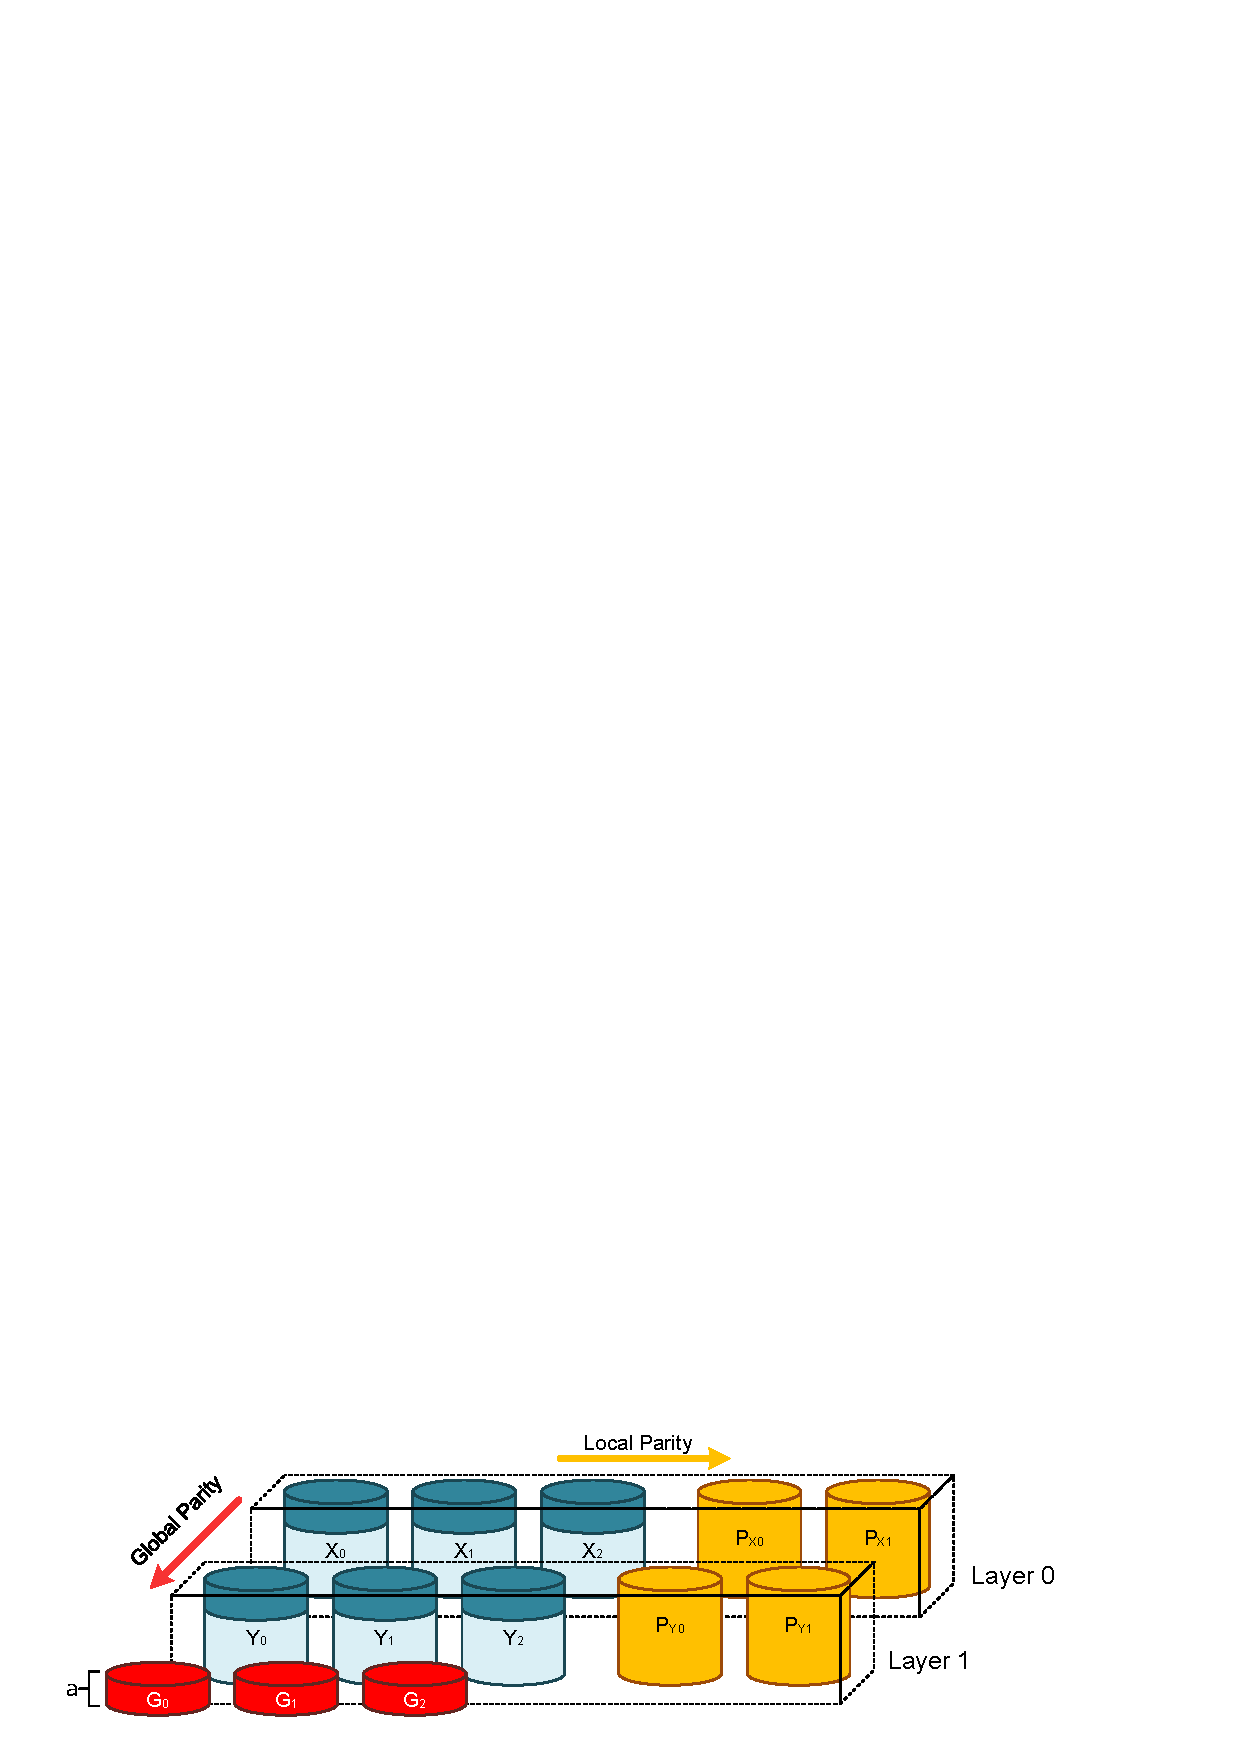
\includegraphics[width=0.45\textwidth]{photo/AP-kmha-v4.pdf}
\caption{A sample of Approximate Codes $(3,2,2,1/3)$ with $h=2$ layers of devices, where each layer contains $k=3$ data devices and $r=2$ parity devices.
The important data occupies $1/3$ of the total data node.
Data nodes are marked as water green and the more important data is marked in darker color. Local parity nodes are marked orange and global parity chunks are marked red.}
\label{fig-Ap-322}
\end{figure}

\subsection{Overview of the Coding Scheme}
\subsubsection{Encoding Process}

The encoding process of Approximate Code is simple, which can be divided into 2 parts: local and global.
The local encoding process takes place in the layer, where data are encoded in node level. In fact, EC methods such as RS-based, XOR-based, MSR, MDS or PMDS codes can all be used to construct the local parity nodes for different advantages.
The global encoding process is independent of the local encoding process and is only for important data. It is designed to encode important data across layers in the simplest way, so we use XOR to generate global parity chunks.
The global parity chunks can be stored in another layer or other nodes. The data layer and the global parity layer can be rotated to avoid uneven distribution of data.

\subsubsection{Decoding Process}
Approximate Code decodes important and unimportant data in different ways. Since the unimportant data is only encoded in local way, its decoding process is on the contrary.
The important data is encoded in both local and global ways, so all the local and global parity chunks are used to decode it, which can be divided into 3 steps:
\begin{enumerate}
\item Inter-layer check, reconstruct data using global parity chunks until it exceeds fault tolerance.
\item In-layer check, reconstruct data using local parity chunks until it exceeds fault tolerance.
\item Inter-layer check again, reconstruct using the global parity chunks.
\end{enumerate}

\subsection{Recovery Mode}

\subsubsection{Full Recovery Mode}
In general, our parameter settings guarantee $h<k$, so the global parity chain is shorter than the local one and has a lower reconstruct overhead.
In addition, the global parity chunks are encoded by XOR, which results in high decoding speed.
Therefore, important data blocks tend to recover data using global parity blocks whenever possible, which makes the Approximate Code have low overall computational overhead and reconstruction costs in \emph{full recovery mode}.

\subsubsection{Approximate Recovery Mode}



\subsection{RS-based Approximate Code}

\subsection{XOR-based Approximate Code}



\subsection{Fault Tolerance}
In this section we give the fault tolerance of important and unimportant data in the Approximate Code.
We first prove the correctness of our decoding process, and then use a program to 
iterate through all the cases of node failures. Finally, we give the data recovery capability of all cases.

For unimportant data, it only has local parity nodes, so its fault tolerance in Approximate Code($k,r,h,a$) is the same as RS($k,r$), which is any $r$ node failures in $k+r$ nodes in each layer.

For important data, We consider the \emph{full recovery mode} and the \emph{approximate recovery mode} separately. When the number of nodes lost per layer does not exceed $r$, the Approximate Code completely recovers all data in \emph{full recovery mode}. If the damage is more severe, the Approximate Code enters the \emph{approximate recovery mode}.


We still take the Approximate Code ($3, 2, 2, 1/3$) as an example, and discuss the fault tolerance of important and mionor data separately.


Important data nodes can tolerate the loss of any 2r+1 data nodes
At the same time tolerate any r+1 node loss. Only in very rare cases, r+2 nodes are damaged in this way, that is, a data node whose local check node and global check node are damaged at the same time.

First consider only the data nodes:
Second, for the case of all nodes:


\iffalse
\subsection{Reconstruct Cost}
In this section, we introduce the recovery overhead for several common failure cases of Approximate Code. The reconstruct cost is defined as the 
\subsubsection{Single node failure}
When any one data node fails, the reconstruction cost of unimportant data is $k$ read and 1 write, while important data has the cost of $h$ read and 1 write. So the total amount of data that needs to be transferred is 
$$ (1-a)*(k+1) + a*(h+1) $$.

For example, when node $X_0$ is lost in case of Approximate Codes $(3,2,2,1/3)$. The amount of data required to rebuild a node is:$\frac{2}{3}*4+\frac{1}{3}*3=\frac{11}{3}$
\fi


\begin{table}[ht]
\centering 
\caption{Comparison of storage overhead and reconstruction cost between Approximate Code, RS and RAID-6.}\label{tab-AS-RS-AP}
\begin{tabular}{|c|c|c|}
\hline
EC & \begin{tabular}[c]{@{}c@{}}Storage\\ Overhead\end{tabular} & \begin{tabular}[c]{@{}c@{}}Reconstruction Cost\\ (single data node failure)\end{tabular} \\ \hline
RS($k,r$) & $\frac{k+r}{k}$ & $k$ \\ \hline
RAID-6($k,2$) & $\frac{k+2}{k}$ & $k$ \\ \hline
\begin{tabular}[c]{@{}c@{}}Ap-Code\\ ($k,r,h,a$)\end{tabular} & $\frac{(k+r)h+ak}{kh}$ & $(1-a)*(k+1) + a*(h+1)$ \\ \hline
\end{tabular}
\end{table}

\subsection{Properties of Approximate Code}

We analyze the nature of the Approximate Code from the following aspects, and the calculation method of the relevant indicators is given in Table \ref{tab-AS-RS-AP}.
\begin{itemize}
    \item Low cost. Approximate code reduces storage overhead by approximating storage strategies. This property is more pronounced for data with a smaller proportion of important data.
    \item High reliability for important data. The Approximate Code guarantees the fault tolerance of the important data $m+s$.
    \item Flexibility. The implementation of the Approximate Code can be based on RS, XOR or a mixture of the two; at the same time, the construction of the Approximate Code can also be used for encoding such as LRC or MSR.
\end{itemize}


\section{Implementation}\label{Implementation}

\begin{figure}[htb]
\centering
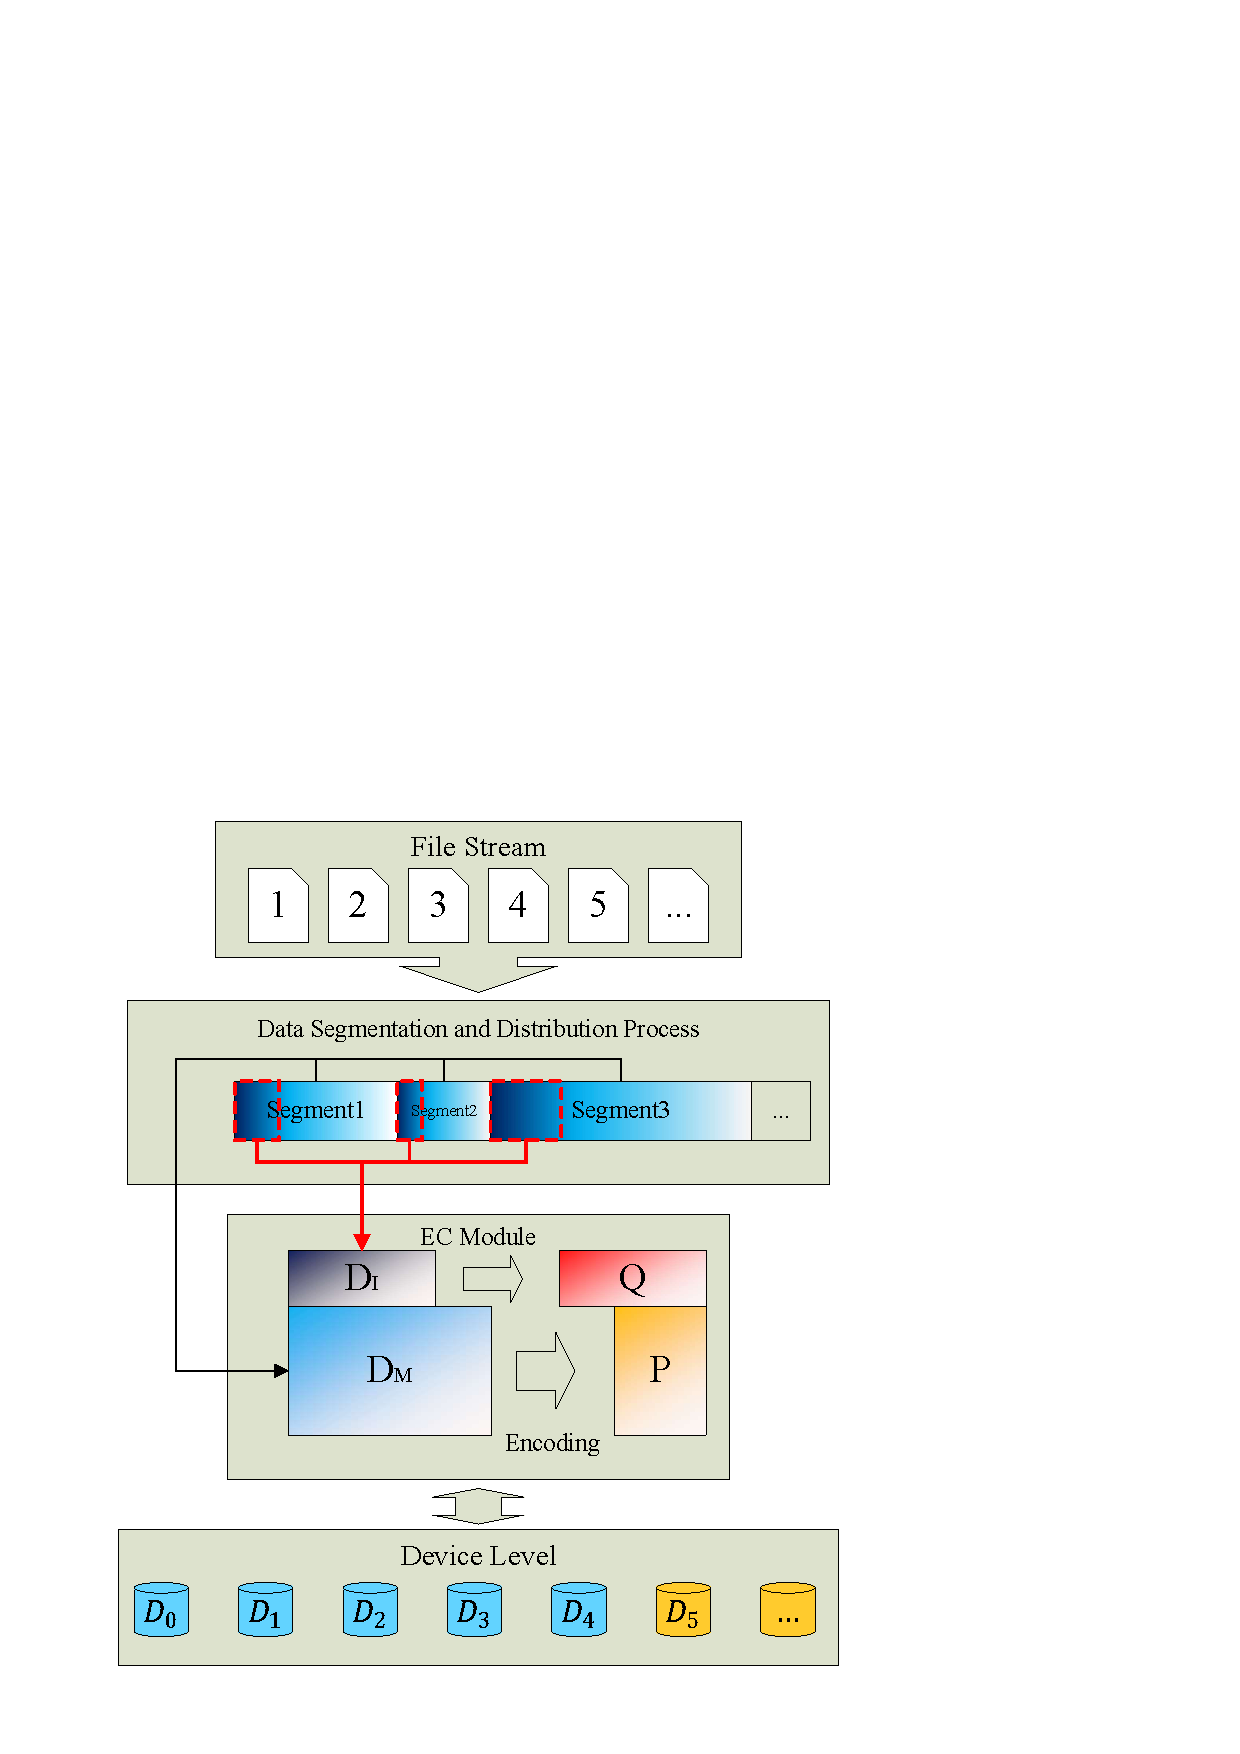
\includegraphics[width=0.4\textwidth]{photo/implementation.pdf}
\caption{Overview of Approximate Code implementation}
\label{fig-implementation}
\end{figure}

Compared with the traditional scheme that does not consider the meaning of the upper layer data, the Approximate Code pays attention to the difference of the importance of the data, so an intermediate layer between the upper layer application and the underlying distributed storage system is necessary to preprocess the data. We call it the approximate storage layer.
The approximate storage layer is responsible for the identification and allocation of data. It controls the EC module and implements the encoding and decoding work of the Approximate Code. 

\subsection{Data Identification}
The identification of data importance can be specified by the upper application as well as automatically determined by the approximate storage layer. We focus on the latter and take video file as an example to introduce our method of automatically distinguishing importance.

For video data encoded by H.264 or similar format, we define I frames as important data, while P frames and B frames as unimportant data based on the analysis in section \ref{video storage}. In practical, video data is rarely stored in the original form of H.264 streams (``.264'' files), but is usually storaged in an file such as ``.mp4'' files containing information such as audio. We transcode video files into raw video streams and other data, and we define these non-video data as important because they contain information that the video can't provide and only take up a small amount of space. The feasibility of this definition will be confirmed in \ref{evaluation}.

\subsection{Data Distribution and Reorganization}
Fortunately, in an H.264 stream, each GOP begins with an I frame followed by a series of P and B frames. Therefore, we store data in units of GOPs. Our main purpose is to store I frames and other frames separately. For non-video data, we distribute it into multiple GOPs and treat it as a special part of the I frame. In the following description, we no longer consider such data especially and simply refer to them as I-frames.
We define $\omega$ as the the important data ratio, which is the size of I-frames divided by the entire GOP size. We also define $\omega_{act}$ as the actual important rate the code can provide by equation \ref{eq-ome-act}.
\begin{equation}\label{eq-ome-act}
    \omega_{act}=\frac{D_I}{D_I+D_M}=\frac{(n-m) \times t}{(n-m) \times r-s \times t}
\end{equation}

  Algorithm \ref{alg-data-dist} and \ref{alg-data-reor} shows the data distribution and reorganization methods.

\begin{algorithm}[htb] 
\caption{Data Distribution Algorithm} 
\label{alg-data-dist} 
\begin{algorithmic}[1] 

\Require  $n$, $m$ and $s$ from the settings of approximate storage layer. Get the type of erasure code.
\Ensure $D_I$, $D_M$, $Q$ and $G$.
\While {true}
\State Divide data into several segments (several GOPs for video data);
\State Calculate $\omega$ of each GOP, and mark the highest one as $\omega_{max}$;
\State Adjust $t$ to find the closest $\omega_{act}$ to $\omega_{max}$;
\Repeat 
\State Divide each GOP into two parts: $\omega_{act}$ and $1-\omega_{act}$;
\State Store the former in $D_I$, the latter in $D_M$;
\Until All GOPs are classified;
\EndWhile

\end{algorithmic} 
\end{algorithm}


\begin{algorithm}[htb] 
\caption{Data Reorganization Algorithm} 
\label{alg-data-reor} 
\begin{algorithmic}[1] 
\Require $D_I$ and $D_M$;
\Ensure A stripe of video data;
\State Find the parameter $(n,m,r,s,t)$ and calculate $\omega_{act}$.
\Repeat
\State Read an I frame from $D_I$ and record its length as $l$.
\State Read $l \times \frac{1-\omega_{act}}{\omega_{act}}$ in $D_M$ and combine two parts.
\Until All blocks are read.
\end{algorithmic} 
\end{algorithm}

The data distribution scheme is shown in the figure \ref{Data-distribution-v2}. We present $\omega_i$ as the $\omega$ of Data(i), and $\omega_{max} = \omega_2$.
For example, Data 3 is represnted by blue, and its key segment (10\%) and part of unimportant segment (10\%) are settled in $D_I$.
The main idea of our data distribution method is to guarantee that each GOP has the same proportion of storage in $D_I$ and $D_M$. This method improves flexibility because it is not necessary to maintain a map that marks the location of each GOP, which makes it is easy to add or delete data at any time. Meanwhile, the method is ideal for streaming video data generated in real time by applications such as monitoring.

\begin{figure}[htb]
\centering
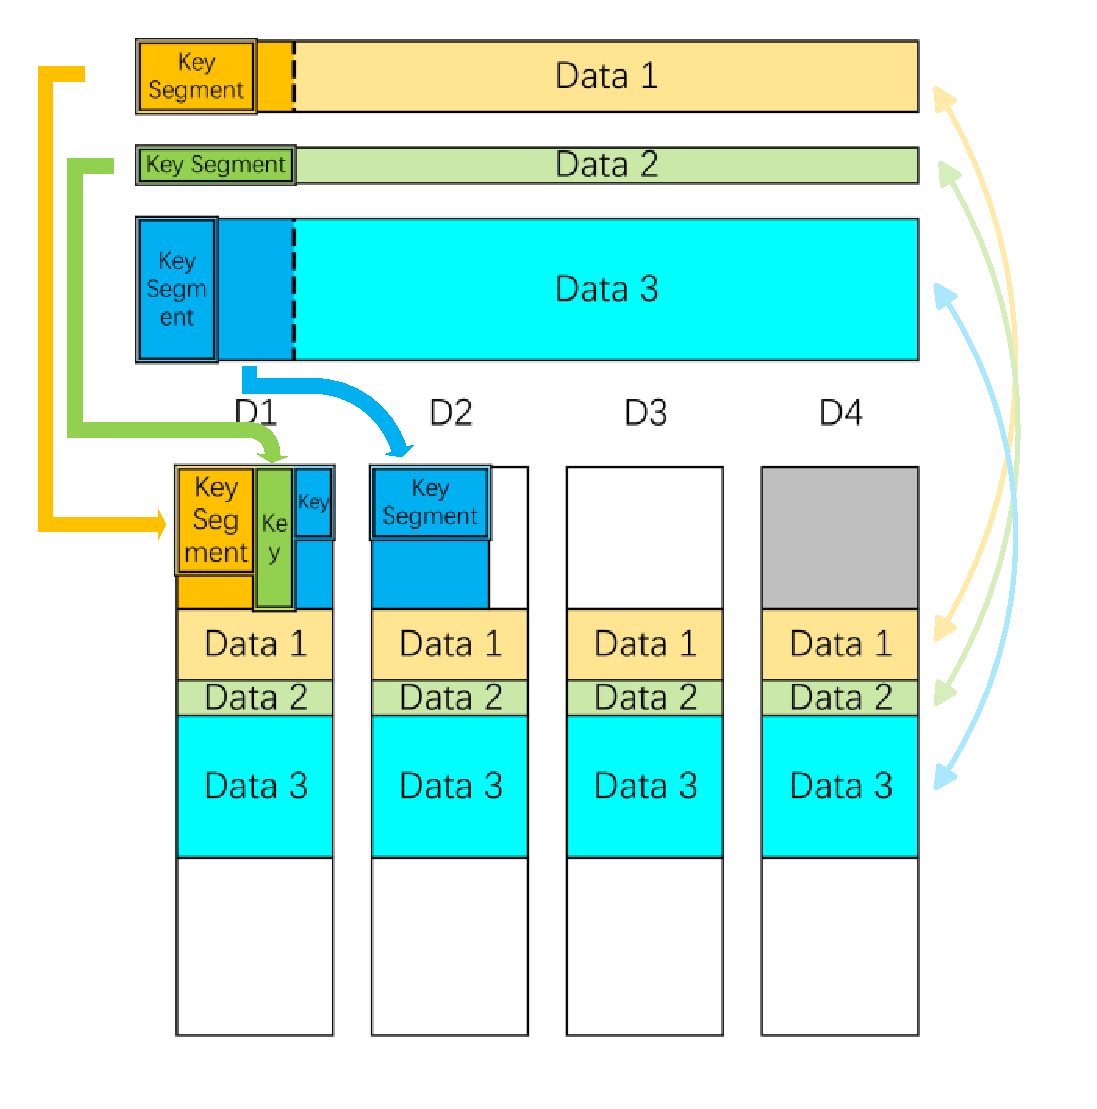
\includegraphics[width=0.32 \textwidth]{photo/Data-distribution-v2.pdf}
\caption{A sample of data distribution method, where the gray block in the upper right corner is the $Q$ area. Here for each data segment, $\omega_1=15\%$, $\omega_2=20\%$ and $\omega_3=10\%$, so the $\omega_{max}=20\%$.}
\label{Data-distribution-v2}
\end{figure}

In addition, our approach can be applied to a variety of other data types. In fact, encoded multimedia data mostly has the property of coexisting important data and non-essential data, such as PTC encoding used in image storage[][].

\section{Experimental Setup}

\subsection{Evaluation methodology}
In our evaluation, we first compare the Approximate Code with the RS code and some XOR-based codes to demonstrate the performance benefits of our solution. Since 3DFTS is a typical erasure code configuration, we use it as a baseline and set the minimum fault tolerance of important data to 3 ($ m + s \geqslant 3 $). We will then demonstrate the quality loss of multimedia data under the traditional and approximate recovery models of severe disk failure to assess the benefits of our approximate storage scheme. We use mathematical analysis and experiments to prove the effectiveness of the Approximate Code.



\subsubsection{Erasure Codes in Our Comparisons}
\textcolor{gray}{
    text text text text text text text text text text text text text text text text text text text text text text text text text text text text text text text text text text text text text text text text text text text text text text text text text text text text text text text text text text text text text text text text text text text text text text text text text text text text text text text text text text text text text text text text text text text text text text text text text text text text text text text text text text text text text text text text text text text text text text text text text text text text text text text text text text text text text text text text text text text text text text text text text text text text text text text text text text text text text text text text text text text text text text text text text text text text text text text text text text text text text text
}

\subsubsection{Platforms and Configurations}
\textcolor{gray}{
    text text text text text text text text text text text text text text text text text text text text text text text text text text text text text text text text text text text text text text text text text text text text text text text text text text text text text text text text text text text text text text text text text text text text text text text text text text text text text text text text text text text text text text text text text text text text text text text text text text text text text text text text text text text text text text text text text text text text text text text text text text text text text text text text text text
}

\subsubsection{Metrics}
\textcolor{gray}{
    text text text text text text text text text text text text text text text text text text text text text text text text text text text text text text text text text text text text text text text text text text text text text text text text text text text text text text text text text text text text text text text text text text text text text text text text text text text text text text text text text text text text text text text text text text text text text text text text text text text text text text text text text text text text text text text text text text text text text text text text text text text text text text text text text text text text text text text text text text text text text text text
}
\subsubsection{Parameters and Assumption in Our Evaluation}
\textcolor{gray}{
    text text text text text text text text text text text text text text text text text text text text text text text text text text text text text text text text text text text text text text text text text text text text text text text text text text text text text text text text text text text text text text text text text text text text text text text text text text text text text text text text text text text text text text text text text text text text text text text text text text text text text text text text text text text text text text text text text text text text text text text text text text text text text text text text text text text text text text text text text text text text text text text text text text text text text text text text text text text text text text text text text text text text text text text text text text text text text text text text text text text text text text
}

\section{Evaluation}\label{evaluation}
This section introduces a series of experiments we have conducted to verify the efficiendy of the Approximate Code.

\begin{table*}[ht]
\centering
\caption{Summary on Various Erasure Codes}
\begin{tabular}{|c|c|c|c|c|c|}
\hline
Name & Fault Tolerance & Storage Overhead & Scalibility & Recovery Cost & \begin{tabular}[c]{@{}c@{}}Computational\\ Complexity\end{tabular} \\ \hline \hline
RS($k,m$) Code & any $m$ disks & $m$ disks & high & high & high \\ \hline
MSR($k,m$) Code & any $m$ disks & $m$ disks & medium & low & very high \\ \hline
Raid 6 & 2 & 2 & low & high & low \\ \hline
SD Code($m,s$) & any $m$ disks and $s$ sectors & $m$ disks and $s$ sectors & low & low & medium \\ \hline
\begin{tabular}[c]{@{}c@{}}Approximate Code($n,m,s,t$)\\ (Important Data)\end{tabular} & any $m+s$ disks & $m$ disks and $s$ sectors & high & high & medium \\ \hline
\begin{tabular}[c]{@{}c@{}}Approximate Code($n,m,s,t$)\\ (unimportant Data)\end{tabular} & any $m$ disks & $m$ disks and $s$ sectors & high & high & high \\ \hline
\end{tabular}
\end{table*}

\begin{table}[htbp]
\begin{tabular}{|c|c|c|c|c|}
\hline
\begin{tabular}[c]{@{}c@{}}Code\\ Config\end{tabular} & \begin{tabular}[c]{@{}c@{}}Storage \\ Overhead\end{tabular} & \begin{tabular}[c]{@{}c@{}}FT\\ (Imp)\end{tabular} & \begin{tabular}[c]{@{}c@{}}FT\\ (unimportant)\end{tabular} & \begin{tabular}[c]{@{}c@{}}Important \\ Rate\end{tabular} \\ \hline
(6,2,4,1,2) & 1.600 & 3 & 2 & 0.200 \\ \hline
(8,2,6,1,1) & 1.371 & 3 & 2 & 0.143 \\ \hline
(10,2,8,1,1) & 1.270 & 3 & 2 & 0.111 \\ \hline
(11,2,9,1,1) & 1.238 & 3 & 2 & 0.100 \\ \hline
(11,3,7,1,1) & 1.400 & 4 & 3 & 0.127 \\ \hline
(13,3,10,1,2) & 1.327 & 4 & 3 & 0.184 \\ \hline
(8,2,6,1,2) & 1.412 & 3 & 2 & 0.294 \\ \hline
(8,2,4,1,2) & 1.455 & 3 & 2 & 0.455 \\ \hline
(10,2,6,2,2) & 1.364 & 4 & 2 & 0.273 \\ \hline
(11,3,8,2,2) & 1.467 & 5 & 3 & 0.200 \\ \hline
\end{tabular}
\end{table}


\subsection{Results}
\textcolor{gray}{
    text text text text text text text text text text text text text text text text text text text text text text text text text text text text text text text text text text text text text text text text text text text text text text text text text text text text text text text text text text text text text text text text text text text text text text text text text text text text text text text text text text text text text text text text text text text text text text text text text text text text text text text text text text text text text text text text text text text text text text text text text text text text text text text text text text text text text text text text text text text text text text text text text text text text text text text text text text text text text text text text text text text text text text text text text text text text text text text text text text text text text text
    text text text text text text text text text text text text text text text text text text text text text text text text text text text text text text text text text text text text text text text text text text text text text text text text text text text text text text text text text text text text text text text text text text text text text text text text text text text text text text text text text text text text text text text text text text text text text text text text text text text text text text text text text text text text text text text text text text text text text text text text text text text text text text text text text text text text text text text text text text text text text text text text text text text text text text text text text text text text text text text text text text text text text text text text text text text text text text text text text text text text text text
}

\subsection{Analysis}
\textcolor{orange}{Illustrate why Approximate Code achieve high reliability with low cost}
\textcolor{gray}{
    text text text text text text text text text text text text text text text text text text text text text text text text text text text text text text text text text text text text text text text text text text text text text text text text text text text text text text text text text text text text text text text text text text text text text text text text text text text text text text text text text text text text text text text text text text text text text text text text text text text text text text text text text text text text text text text text text text text text text text text text text text text text text text text text text text text text text text text text text text text text text text text text text text text text text text text text text text text text text text text text text text text text text text text text text text text text text text text text text text text text text text
    text text text text text text text text text text text text text text text text text text text text text text text text text text text text text text text text text text text text text text text text text text text text text text text text text text text text text text text text text text text text text text text text text text text text text text text text text text text text text text text text text text text text text text text text text text text text text text text text text text text text text text text text text text text text text text text text text text text text text text text text text text text text text text text text text text text text text text text text text text text text text text text text text text text text text text text text text text text text text text text text text text text text text text text text text text text text text text text text text text text text text text text text text text text text text text text text text text text text text text text text text text text text text text text text text text text text text text text text text text text text text text text text text text text text text text text text text text text text text text text text text text text text text text text text text text text text text text text text text text text text text text text text text text text text text text text text text text text text text text text text text text text text text text text text text text text text text text text text text text text text text text text text text text text text text text text text text text text text text text text text text text text text text text text text text text text text text text text text text text text text text text text text text text text text text text text text text text text text text text text text text text text text
    text text text text text text text text text text text text text text text text text text text text text text text text text text text text text text text text text text text text text text text text text text text text text text text text text text text text text text text text text text text text text text text text text
}


\section{Conclusion}\label{Conclusion}

\textcolor{gray}{
    text text text text text text text text text text text text text text text text text text text text text text text text text text text text text text text text text text text text text text text text text text text text text text text text text text text text text text text text text text text text text text text text text text text text text text text text text text text text text text text text text text text text text text text text text text text text text text text text text text text text text text text text text text text text text text text text text text text text text text text text text text text text text text text text text text text text text text text text text text text text text text text text text text text text text text text text text text text text text text text text text text text text text text text text text text text text text text text text text text text text text text
    text text text text text text text text text text text text text text text text text text text text text text text text text text text text text text text text text text text text text text text text text text text text text text text text text text text text text text text text text text text text text text text text text
}


\begin{acks}

\end{acks}



\bibliographystyle{ACM-Reference-Format}
\bibliography{ApproximateCode}

\end{document}
